\documentclass[10pt,a4paper]{article}
\usepackage{fontspec}
\defaultfontfeatures{Mapping=tex-text}
\usepackage{xunicode}
\usepackage{xltxtra}
%\setmainfont{???}
\usepackage{xeCJK}
\usepackage{ctex}
\usepackage{polyglossia}
\setdefaultlanguage{english}
\usepackage{indentfirst}
\setlength{\parindent}{2em}%中文缩进两个汉字位
\usepackage{amsmath}
\usepackage{amsfonts}
\usepackage{amssymb}
\usepackage{siunitx}
\usepackage{float}

\usepackage{cite}

\usepackage{amsmath}
 \usepackage{siunitx}
\usepackage{geometry}

\author{翁俊}
\title{江门中微子实验(JUNO)调研报告}

\begin{document}

\maketitle
\newpage
\tableofcontents
\newpage

\section{JUNO实验课题背景与研究目标}

江门中微子实验是是继大亚湾反应堆中微子实验之后由中国主持的第二个大型中微子实验。实验站将建在地下700米深处,实验计划最早在2021年投入运行并开始物理取数,运行至少20年。实验建造的中微子探测器将是世界上能量精度最高、规模最大的液体闪烁体探测器。这一实验的启动标志着我国中微子实验研究从起步到跨越的转变。

	
\subsection{神奇的幽灵粒子}
中微子,又译作微中子,是轻子的一种,是组成自然界的最基本的粒子之一,常用符号$\nu$表示。中微子不带电,自旋为1/2,质量非常轻(有的小于电子的百万分之一),以接近光速运动。



粒子物理的研究结果表明,构成物质世界的最基本的粒子有12种,包括6种夸克,3种带电轻子(电子,$\mu $子和$\tau$子)和3种中微子(电子中微子,$\mu$中微子和$\tau$中微子),其各自的位置如Figure \ref{fig:0}所示:
%\cite{}

\begin{figure}[H]
 \centering
 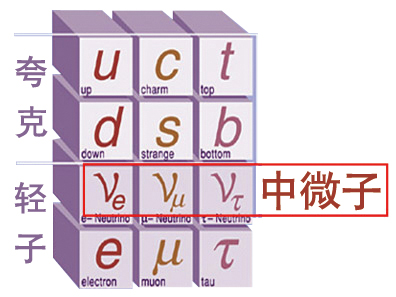
\includegraphics[height=5cm]{images/standarmodel.jpg}
 \caption{标准模型示意图:}
 \label{fig:0}
\end{figure}

中微子个头小,不带电,可自由穿过地球,与其他物质的相互作用十分微弱,号称宇宙间的"隐身人"。科学界从预言它的存在到发现它,用了20多年的时间。

目前标准模型中认为,3种中微子(电子中微子,$\mu$中微子和$\tau$中微子)是构成物质世界的最基本的十二种粒子之三,三种中微子味道中微子如下:

每一种中微子都对应一种带电的轻子——电子中微子对应电子,$\mu$中微子对应$\mu$子,同理,$\tau$中微子对应$\tau$子。

\newpage
%----------------------------------SYSTEM DESIGN------------------------------------------

\subsection{中微子振荡}\label{sub:sysover}


中微子振荡(Neutrino oscillation)是一个量子力学现象,是指中微子在生成时所伴随的轻子(包括电子,$\mu$子和$\tau$子)味可在之后转化成不同的味,而被测量出改变。当中微子在空间中传播时,自发的会发生味道的周期性变化。

自然界中存在三种中微子,即电子中微子,μ中微子和τ中微子,分别对应了参与带电流弱相互作用的带电轻子。中微子振荡的验证了一种类型的中微子在传播一段距离后会变成另外一种类型的中微子。对这种现象的解释为三种中微子具有不同的静止质量且存在轻子混合态。换一种说法即是在传播过程中,中微子存在三种质量的本征态,分别对应了三个质量。如果存在轻子味道的混合,那么味道的本征态和质量的本征态就不会是一样的。当某弱相互作用产生中微子时,中微子的状态应该是三个量子本征态的叠加态,在传播的过程中,表现为质量本征态的相干叠加,当经过一段距离后,质量的本征态之间会产生一定的相位差,导致到达探测器中的中微子的状态和产生时的状态不一致。因此,可以将中微子振荡理解为具有本征态质量的中微子呈现出来的一种宏观相干叠加现象。一个简单的中微子振荡示意图如Figure \ref{fig:10}。


\begin{figure}[H]
 \centering
 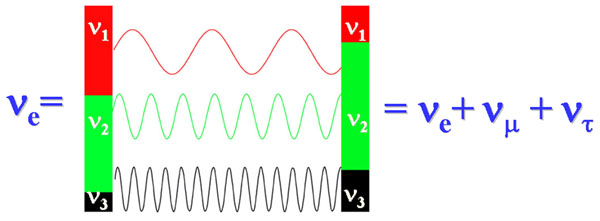
\includegraphics[height=4cm]{images/中微子振荡示意图.jpg}
 \caption{一个简单的中微子振荡图像表述\cite{pic1}}
 \label{fig:10}
\end{figure}

接下来,本文将对中微子振荡进行一定的推导\cite{2007fun}\cite{2016Neutrino}\cite{2019Physics}:


中微子的弱相互作用本征态可以写为:$\nu_{\alpha}$,其中,$\alpha=e,\mu,\tau$,而质量的本征态可以写为$\nu_{i}$,其中,$i=1,2,3$。中微子混合矩阵(MNSP矩阵)描述了质量本征态和弱作用本征态之间的转化关系。三代中微子混合的MNSP矩阵U描述的转化关系如下:
\begin{equation}
\label{con:eq1}
\begin{pmatrix}
 \nu_e  \\
 \nu_{\mu}  \\
 \nu_{\tau}
 \end{pmatrix}
 =U \begin{pmatrix}
 \nu_1  \\
 \nu_2  \\
 \nu_3
 \end{pmatrix}
 = \begin{pmatrix}
 1 & 0 & 0 \\
 0 & c_{23} & s_{23} \\
 0 & -s_{23} & c_{23}
 \end{pmatrix}
 \begin{pmatrix}
 c_{13} & 0 & s_{13}e^{i\delta} \\
 0 & 1 & 0 \\
 -s_{13}e^{i\delta} & 0 & c_{13}
 \end{pmatrix} 
 \begin{pmatrix}
 c_{12} & s_{12} & 0 \\
 -s_{12} & c_{12} & 0 \\
 0 & 0 & 1
 \end{pmatrix}
 \begin{pmatrix}
 \nu_1  \\
 \nu_2  \\
 \nu_3
 \end{pmatrix}
\end{equation}


其中,$c_{ij}=\cos{\theta_{ij}}$,$s_{ij}=\sin{\theta_{ij}}$,$\delta$为CP破坏的相角\cite{2009Experimental}。


则态$\nu_{\alpha}$可以表示为质量态的叠加:
\begin{equation}
\label{con:eq2}
|\nu_{\alpha}\rangle=\sum_{k}U_{\alpha k}^{*}|\nu_{k}\rangle
\end{equation}


本征态满足归一化条件:
\begin{equation}
\label{con:eq3}
\begin{split}
\langle \nu_{\alpha}|\nu_{\beta}\rangle=\delta_{\alpha\beta}\\
\langle\nu_{i}|\nu_{j}\rangle=\delta_{ij}
\end{split}
\end{equation}


质量的本征态满足Hamitonian方程:
\begin{equation}
\label{con:eq4}
H_{0}|\nu_{k}\rangle=E_{k}|\nu_{k}\rangle
\end{equation}


其中:$E_{k}^2=p^2+m_{k}^2$,p为中微子的动量,$m_{k}$为中微子的静止质量。


因此,薛定谔方程可以写为:
\begin{equation}
\label{con:eq5}
i\frac{\partial}{\partial t}|\nu_{k}\rangle=H_{0}|\nu_{k}\rangle
\end{equation}


其解为:
\begin{equation}
\label{con:eq6}
|\nu_{k}(t)\rangle=e^{-iE_{k}t}|\nu_{k}\rangle
\end{equation}


带入到式\eqref{con:eq2}:
\begin{equation}
\label{con:eq7}
|\nu_{\alpha}(t)\rangle=\sum_{k}U_{\alpha k}^{*}|\nu_{k}(t)\rangle=\sum_{k}U_{\alpha k}^{*}e^{-iE_{k}t}|\nu_{k}\rangle
\end{equation}


做一个初始条件的约定:
\[|\nu_{k}\rangle=|\nu_{k}(0)\rangle\]


而式\eqref{con:eq2}的逆变换可以写为:
\begin{equation}
\label{con:eq8}
|\nu_{k}\rangle=\sum_{k}U_{\alpha k}|\nu_{\alpha}\rangle
\end{equation}


带入到式\eqref{con:eq6}并用$\beta$代替$\alpha$:
\begin{equation}
\label{con:eq9}
|\nu_{k}(t)\rangle=\sum_{\beta}U_{\beta k}^{*}e^{-iE_{k}t}|\nu_{\beta}\rangle
\end{equation}


结合式\eqref{con:eq6}\eqref{con:eq8},可以得到:
\begin{equation}
\label{con:eq10}
|\nu_{\alpha}(t)\rangle=\sum_{k,\alpha}U_{\alpha k}^{*}U_{\beta k}e^{-iE_{k}t}|\nu_{\beta}\rangle
\end{equation}


由此,t时刻的中微子的态可以表示为初始时刻的本征态的叠加.从态$|\alpha\rangle$振荡到态$|\beta\rangle$的幅度为:
\begin{equation}
\label{con:eq11}
A_{\alpha\beta}(t)=\langle\beta|\alpha(t)\rangle=\sum_{k}U_{\alpha k}^{*}U_{\beta k}e^{-iE_{k}t}
\end{equation}


从态$|\alpha\rangle$振荡到态$|\beta\rangle$的概率为:
\begin{equation}
\label{con:eq12}
\begin{split}
P_{\alpha\beta}(t)=A_{\alpha\beta}(t){A_{\alpha\beta}(t)}^*=\sum_{k,j}U_{\alpha k}^{*}U_{\beta k}e^{-iE_{k}t}U_{\alpha j}^{*}U_{\beta j}e^{iE_{j}t}\\
=\sum_{k,j}U_{\alpha k}^{*}U_{\beta k}U_{\alpha j}U_{\beta j}^{*}e^{-i(E_{k}-E_{j})t}
\end{split}
\end{equation}


中微子的运动速度是很接近光速的,是相对论粒子的范畴,动能远大于静止能量,因此,对于其能量可以做一个近似:
\begin{equation}
\label{con:eq13}
E_{k}=\sqrt{p^2+m_k^2}=|p|\sqrt{1+\frac{m_k^2}{p^2}}\approx |p|+\frac{m_k^2}{2|p|}=E+\frac{m_k^2}{2E}
\end{equation}


其中,$E=|q|$。
带入到式\eqref{con:eq12}:
\begin{equation}
\label{con:eq14}
P_{\alpha\beta}(t)=\sum_{k,j}U_{\alpha k}^{*}U_{\beta k}U_{\alpha j}U_{\beta j}^{*}e^{-i\frac{\Delta m_{kj}^2}{2E}t}
\end{equation}


$\Delta m_{kj}^2=m_k^2-m_j^2$表示的是中微子质量本征态的质量平方的差。


在自然单位中,光速c的量纲为1,近似认为中微子速度为c,在t是时刻传播的距离为L,带入到式\eqref{con:eq14}:
\begin{equation}
\label{con:eq15}
P_{\alpha\beta}(t)=\sum_{k,j}U_{\alpha k}^{*}U_{\beta k}U_{\alpha j}U_{\beta j}^{*}e^{-i\frac{\Delta m_{kj}^2}{2E}L}
\end{equation}


带入欧拉公式展开,可将实部和虚部分开,同时根据k和j的大小关系可分为三部分,其中,k和j交换位置后的值应该是相等的,所以有:
\begin{equation}
\label{con:eq16}
\begin{split}
P_{\alpha\beta}(L)&=\sum_{k=j}U_{\alpha k}^{*}U_{\beta k}U_{\alpha j}U_{\beta j}^{*}e^{-i\frac{\Delta m_{kj}}{2E}L}+\sum_{k,j |k<j}U_{\alpha k}^{*}U_{\beta k}U_{\alpha j}U_{\beta j}^{*}e^{-i\frac{\Delta m_{kj}}{2E}L}
\\&+\sum_{k,j |k>j}U_{\alpha k}^{*}U_{\beta k}U_{\alpha j}U_{\beta j}^{*}e^{-i\frac{\Delta m_{kj}}{2E}L}
\\&=\sum_{k}{|U_{\alpha k}|}^{2}{|U_{\beta k}|}^{2}+2\sum_{k,j |k>j}U_{\alpha k}^{*}U_{\beta k}U_{\alpha j}U_{\beta j}^{*}\cos(\frac{\Delta m_{kj}}{2E}L)
\\&+2\sum_{k,j |k>j}iU_{\alpha k}^{*}U_{\beta k}U_{\alpha j}U_{\beta j}^{*}\sin(-\frac{\Delta m_{kj}}{2E}L)
\\&=\sum_{k}{|U_{\alpha k}|}^{2}{|U_{\beta k}|}^{2}+2\sum_{k,j |k>j}{\rm Re}[U_{\alpha k}^{*}U_{\beta k}U_{\alpha j}U_{\beta j}^{*}\cos(\frac{\Delta m_{kj}}{2E}L)]
\\&-2\sum_{k,j |k>j}{\rm Im}[U_{\alpha k}^{*}U_{\beta k}U_{\alpha j}U_{\beta j}^{*}\sin(-\frac{\Delta m_{kj}}{2E}L)]
\end{split}
\end{equation}


其中:\begin{equation}
\label{con:eq17}
\sum_{k}{|U_{\alpha k}|}^{2}{|U_{\beta k}|}^{2}=\delta_{\alpha\beta}-2{\rm Re}\sum_{k,j |k>j}U_{\alpha k}^{*}U_{\beta k}U_{\alpha j}U_{\beta j}^{*}
\end{equation}


结合余弦函数的二倍角公式,得到:
\begin{equation}
\label{con:eq18}
\begin{split}
P_{\alpha\beta}(L)&=\delta_{\alpha\beta}-2{\rm Re}\sum_{k,j |k>j}U_{\alpha k}^{*}U_{\beta k}U_{\alpha j}U_{\beta j}^{*}+2\sum_{k,j |k>j}{\rm Re}[U_{\alpha k}^{*}U_{\beta k}U_{\alpha j}U_{\beta j}^{*}\cos(\frac{\Delta m_{kj}}{2E}L)]\\&-2\sum_{k,j |k>j}{\rm Im}[U_{\alpha k}^{*}U_{\beta k}U_{\alpha j}U_{\beta j}^{*}\sin(-\frac{\Delta m_{kj}}{2E}L)]
\\
&=\delta_{\alpha\beta}-4\sum_{k,j |k>j}{\rm Re}[U_{\alpha k}^{*}U_{\beta k}U_{\alpha j}U_{\beta j}^{*}\sin^2(\frac{\Delta m_{kj}}{4E}L)]
\\&+\sum_{k,j |k>j}{\rm Im}[U_{\alpha k}^{*}U_{\beta k}U_{\alpha j}U_{\beta j}^{*}\sin(\frac{\Delta m_{kj}}{2E}L)]
\end{split}
\end{equation}


而式\eqref{con:eq1}中MNSP矩阵的形式可以写为:
\begin{equation}
\label{con:eq19}
\begin{aligned}
U &= \begin{pmatrix}
 1 & 0 & 0 \\
 0 & c_{23} & s_{23} \\
 0 & -s_{23} & c_{23}
 \end{pmatrix}
 \begin{pmatrix}
 c_{13} & 0 & s_{13}e^{i\delta} \\
 0 & 1 & 0 \\
 -s_{13}e^{i\delta} & 0 & c_{13}
 \end{pmatrix} 
 \begin{pmatrix}
 c_{12} & s_{12} & 0 \\
 -s_{12} & c_{12} & 0 \\
 0 & 0 & 1
 \end{pmatrix}
 \\&=
 \begin{pmatrix}
 c_{12}c_{13} & s_{12}c_{13} & s_{13}e^{-i \delta} \\
 -s_{12}c_{23}-c_{12}s_{23}s_{13}e^{i\delta} & c_{12}c_{23}-s_{12}s_{23}s_{13}e^{i\delta} & s_{23}c_{13} \\
 s_{12}c_{23}-c_{12}c_{23}s_{13}e^{i\delta} &-c_{12}s_{23}-c_{12}c_{23}s_{13}e^{i\delta} & c_{23}c_{13}
 \end{pmatrix}
 \end{aligned}
\end{equation}
其中,$c_{ij}=cos\theta_{ij},s_{ij}=sin\theta_{ij}$。


从展开式中可以得到,虚部可以表示为:
\begin{equation}
\label{con:eq20}
{\rm Im}[U_{\alpha k}^{*}U_{\beta k}U_{\alpha j}U_{\beta j}]=s_{\alpha \beta kj}J
\end{equation}


其中,$s_{\alpha \beta kj}\in {0,1,-1}$,J是表征CP破坏程度的观测量:
\[
J=\sin\delta s_{12}c_{12}s_{13}c_{13}^2 s_{23}c_{23}
\]


因此,式\eqref{con:eq18}可以改写为:
\begin{equation}
\label{con:eq21}
\begin{aligned}
P_{\alpha\beta}(L)&=\delta_{\alpha\beta}-4\sum_{k,j |k>j}{\rm Re}[U_{\alpha k}^{*}U_{\beta k}U_{\alpha j}U_{\beta j}^{*}\sin^2(\frac{\Delta m_{kj}}{4E}L)]
\\&+2J\sum_{k,j |k>j}s_{\alpha \beta kj}\sin(\frac{\Delta m_{kj}}{2E}L)]
\end{aligned}
\end{equation}


式\eqref{con:eq21}中的${\rm Re}[U_{\alpha k}^{*}U_{\beta k}U_{\alpha j}U_{\beta j}^{*}]$与$s_{\alpha \beta kj}$各项可在文献\cite{2007fun}中Tab.13.1中找到。至此,就已经得到了中微子经过距离L后的存活概率。同时,可以从式(19)的表达式中看出,由质量的平方差值决定的中微子振荡的观测可以用于确定振荡角。


在JUNO实验中,测量的主要是反应堆中微子的存活概率。取$\alpha=\beta=\bar{\nu_e}$
得到:
\begin{equation}
\label{con:eq22}
\begin{split}
P(\bar{\nu_e}\rightarrow\bar{\nu_e})&=1-4\sum_{k,j |k>j}U_{e k}^{*}U_{e k}U_{e j}U_{e j}^{*}\sin^2(\frac{\Delta m_{kj}}{4E}L)
\\&=1-4\sum_{k,j |k>j}|U_{e k}|^2|U_{e j}|^2\sin^2(\frac{\Delta m_{kj}}{4E}L)
\end{split}
\end{equation}


将MNSP矩阵带入到式\eqref{con:eq22},得到:
\begin{equation}
\label{con:eq23}
\begin{split}
P(\bar{\nu_e}-\bar{\nu_e},L)&=1-{\sin^2{2\theta_{12}}} c_{13}^4\sin^2{\frac{\Delta{m_{21}^2}L}{4E}}\\&-
\sin^2{2\theta_{13}} c_{12}^2\sin^2{\frac{\Delta{m_{31}^2}L}{4E}}
\\&-\sin^2{2\theta_{13}} s_{12}^2\sin^2{\frac{\Delta{m_{32}^2}L}{4E}}
\end{split}
\end{equation}


从反中微子的存活概率来看,不包含CP破坏相角$\delta$,在避免了CP破坏相角带来的测量问题的同时,也损失了测量CP破坏相角的可能性。

\newpage
\subsection{中微子的质量}\label{sub:sysover}

中微子振荡实验证明了中微子是有质量的,且存在味道的混合。在振荡实验中,已经精确测量了两个独立的中微子质量平方差的值,但目前仍然对于三者的质量大小仍然是未知的。


振荡实验只能得到质量的平方顺序,无法给出绝对质量的信息。德国的卡尔斯鲁厄氚中微子(KATRIN)实验通过测量$\beta$衰变的电子能谱终点来限制中微子质量,于2018年6月11日正式开始运行,是目前最灵敏的中微子“体重计”,在进行足够的采数后,将会给出更加精确的中微子的质量上限。

宇宙微波背景辐射和大尺度结构的观测,因为有质量的中微子会影响宇宙的演化。PLANCK实验组的最新观测结果显示三个中微子质量之和的上限为\SI{0.23}{eV}(0.95置信度),由此可以看出中微子的绝对质量不超过\SI{0.1}{eV}\cite{plank}。

\newpage
\section{JUNO实验综述} \label{sysdes}%------------------------------

\subsection{JUNO中的中微子物理}\label{sub:sysover}
\subsubsection{中微子的质量顺序}\label{sub:sysover}

中微子振荡现象的发现确定了中微子的质量不为0,目前,标准的中微子的三味振荡的研究现状如下\cite{2016Neutrino}:
\begin{itemize}
	\item{中微子MNSP轻子混合矩阵中三个非零混合角在精度在4\%到10\%得到了测量。}
    \item{中微子两个独立的质量平方差的大小已经测量,且测量精度优于4\%。}
    \item{目前测出的中微子质量平方差其中一个差得到的仅为其大小,对于其中的正负号仍然未知,因此,第三代中微子和前两代中微子的质量大小顺序是未知的。$\Delta m_{21}^2=m_{2}^2-m_{1}^2;|\Delta m_{31}^2|=|m_{3}^2-m_{1}^2|$}
    \item{轻子CP破坏中,在MNSP矩阵中的CP破坏相角$\delta$ 未知。}
\end{itemize}

因此,测量中微子的质量顺序和CP破坏相角是未来一段时间内的重点。而JUNO实验的设计建设运行,将会给出中微子质量顺序的答案。

以下为JUNO实验测量中微子质量顺序(The neutrino mass hierarchy,简称MH)的原理\cite{2016Neutrino}:

第三代中微子的质量和前面两代的质量相比,有两种可能的情况:第一种是认为第三代中微子的质量比第二代、第一代中微子的质量大(The normal mass hierarchy,简称NH);第二种则是认为第三代中微子的质量比前两代中微子的质量小(The Inverted mass hierarchy,简称IH)。
由中微子振荡的理论推导,可以得到\cite{Ternes:2020bvy}:
\begin{equation}
 \begin{split}
    \label{con:eq30}
     P(\bar{\nu_e}-\bar{\nu_e},L)=1-{\sin^2{2\theta_{12}}} c_{13}^4\sin^2{\frac{\Delta{m_{21}^2}L}{4E}}-\\
\sin^2{2\theta_{13}}[c_{12}^2\sin^2{\frac{\Delta{m_{31}^2}L}{4E}}+s_{12}^2\sin^2{\frac{\Delta{m_{32}^2}L}{4E}}]
 \end{split}
\end{equation}


式\eqref{con:eq30}可写为:
 \begin{equation}
 \label{con:eq24}
 \begin{split}
     P(\bar{\nu_e}-\bar{\nu_e},L)=1-\frac{1}{2}{\sin^2{2\theta_{13}}}[1-\sqrt{1-\sin^2{2\theta_{12}}}\sin^2{\Delta_{21}}\\\cos(2|\Delta_{ee}|\pm\phi)] -\cos^4{\theta_{13}}\sin^2{2\theta_{12}}\sin^2{\Delta_{21}} 
 \end{split}
 \end{equation}

其中:
\[
\begin{split}
&\Delta_{ij}=\frac{\Delta{m_{ij}^2}L}{4E}\\
&\Delta_{ee}=\Delta{m_{ee}^2}=\sin^2{\theta_{12}}\Delta{m_{31}^2}-\cos^2{\theta_{12}}\Delta{m_{32}^2}\\
&\sin\phi=\frac{c_{12}^2\sin(2s_{12}^2\Delta_{21})-s_{12}^2\sin(2c_{12}^2\Delta_{21})}{\sqrt{1-\sin^2\theta_{12}\sin^2\Delta_{21}}}\\&\cos\phi=\frac{c_{12}^2\cos(2s_{12}^2\Delta_{21})+s_{12}^2\cos(2c_{12}^2\Delta_{21})}{\sqrt{1-\sin^2\theta_{12}\sin^2\Delta_{21}}}
\end{split}
\]
L代表了中微子实验的基线长度,E为所测量的反电子中微子的能量。


定义:$\Delta{m_{\phi}^2}=\frac{4E\phi}{L}$

则对于NH而言,中微子的质量平方差可以表示为:$2|\Delta{m_{ee}^2}|+\Delta{m_{\phi}^2}$,对于IH而言则可以表示为:$2|\Delta{m_{ee}^2}|-\Delta{m_{\phi}^2}$。这就使得NH和IH得到的振荡信号有所差异。这种差异的显著程度与中微子的动能和传播距离有关,Figure \ref{fig:11}给出了其的相关关系:
\begin{figure}[H]
 \centering
 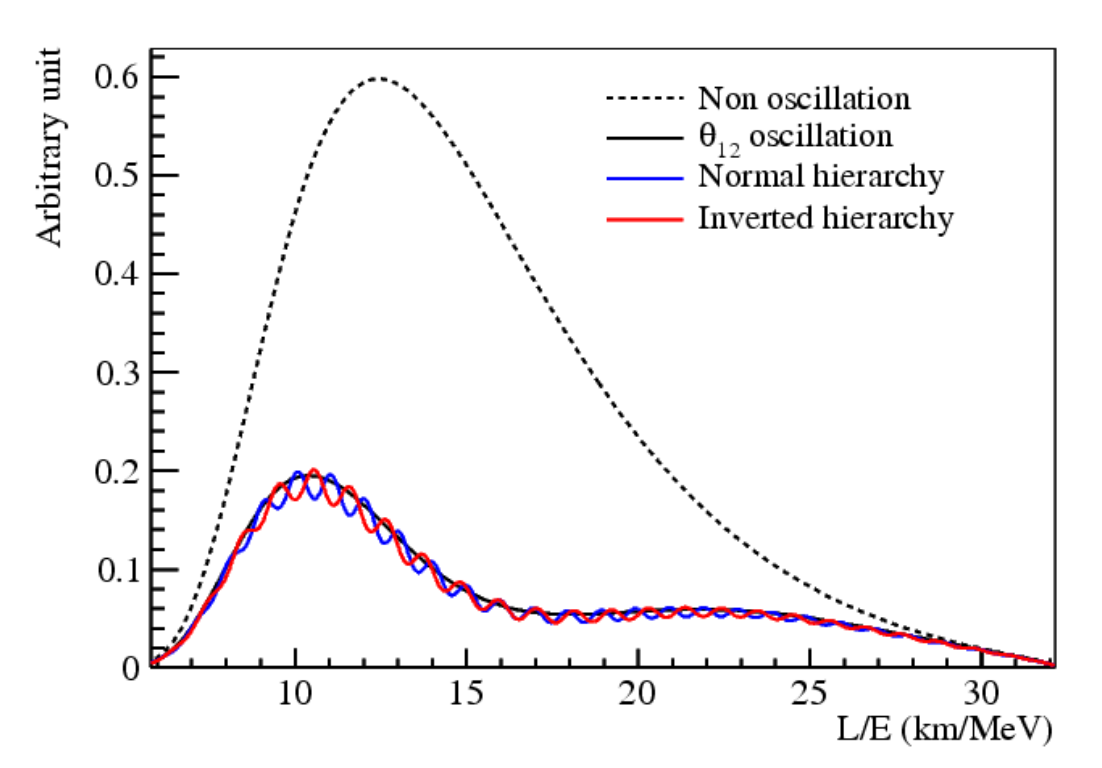
\includegraphics[height=8cm]{images/L-selet.png}
 \caption{为中微子存活概率与E/L的关系\cite{2016Neutrino}}
 \label{fig:11}
\end{figure}


JUNO实验前期采用了最小二乘法来表征质量顺序的敏感程度,建立的卡方函数如式\eqref{con:eq30}:
\begin{equation}
 \label{con:eq30}
 \begin{split}
    \chi_{REA}^2=\Sigma_{i=1}^{N_{bin}}\frac{[M_i-T_i(1+\Sigma_{k}\alpha_{ik} \epsilon_{k})]^2}{M_{i}}+\Sigma_{k}
\frac{\epsilon_k^2}{\sigma_k^2} 
\end{split}
 \end{equation}

其中,$M_i$为能量处在第i个bin中的事例数,$T_i$为预测的第i个bin中的事例数,$\sigma_k$描述的是系统不确定度,$\alpha_{ik}$表示第k个特征对中微子事例在第i个能量区间的影响,$\epsilon_k$则对应于所有特征的影响。对\SI{1.8}{MeV}到\SI{8}{MeV}的中微子进行模拟,拟合IH谱和NH谱,以$\Delta\chi_{MH}^2=|\chi_{min}(NH)^2-\chi_{min}(IH)^2|
$作为MH的敏感程度,得到如Figure \ref{fig:21}的结果\cite{2016Neutrino}:


\begin{figure}[H]
 \centering
 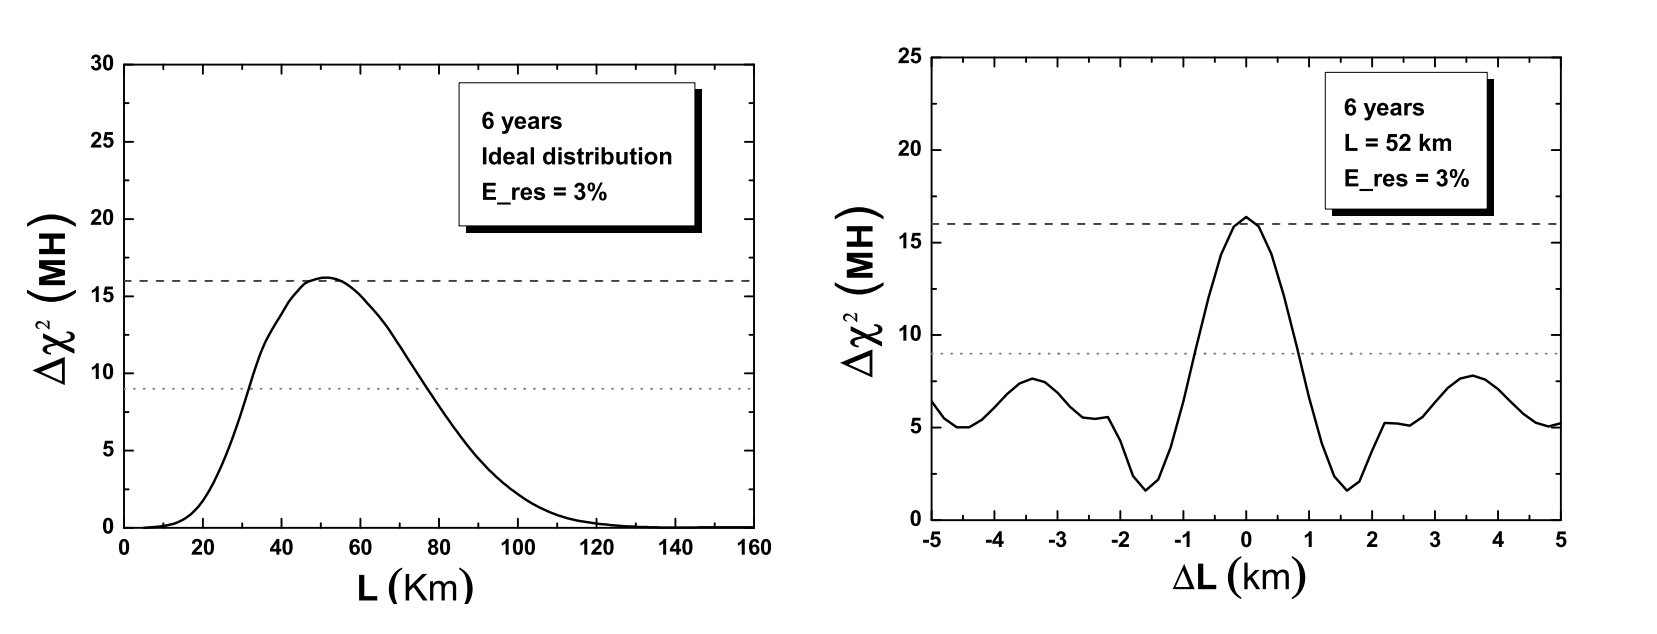
\includegraphics[height=7cm]{images/L-selet1.png}
 \caption{模拟6年采数后MH对基线长度($L$)的敏感程度(图左)和对两个核电站的距离之差的敏感程度($\Delta L$),从左图可知,探测器建在距离核电站\SI{50}{km}左右时,MH的敏感程度是最高的;从右图可知,两个核电站到实验点的距离之差$\Delta L=0$时,MH的敏感程度最高。}
 \label{fig:21}
\end{figure}



从式(20)可以看出,中微子的存活概率可以分为以下三个部分\cite{Zhan:2008id}:
 \begin{equation}
 \label{con:eq25}
 \begin{split}
P(\bar{\nu_e}-\bar{\nu_e},L)=1-P_{21}-P_{31}-P_{31}\\
P_{21}=\cos^4{\theta_{13}}\sin^2{2\theta_{12}}\sin^2{\Delta_{21}}\\
P_{31}=\cos^2{\theta_{12}}\sin^2{2\theta_{13}}\sin^2{\Delta_{31}}\\
P_{32}=\sin^2\theta_{13}\sin^2{2\theta_{13}}\sin^2{\Delta_{32}} 
 \end{split}
 \end{equation}

可以看出,反电子中微子的存活概率可以描述为$1-P_{21}$、$P_{31}$、$P_{32}$的线性叠加,同时,$1-P_{21}$不涉及到质量顺序相关的项,对MH不敏感;$P_{31}$、$P_{32}$依赖于质量的排序,对于IH和NH的细微差别有明显的不同。

在JUNO探测器中,探测到的中微子的数量,除了与存活概率相关之外,还会与发射中微子的能谱和反应截面有关,将中微子的存活概率等视为$\frac{L}{E}$的分布谱,则可以用下式描述探测到的反电子中微子的$\frac{L}{E}$谱:
\begin{equation}
\label{con:eq26}
F(\frac{L}{E})=\phi(E)\sigma(E)P_{\bar{\nu_e}\rightarrow\bar{\nu_e}}(\frac{L}{E})
\end{equation}

其中,$\phi(E)$描述的是中微子的发射谱,即来自于反应堆中不同反应中对应于能量E的发射;$\sigma(E)$描述的是探测器探测到中微子的反应截面。

给定傅里叶的正余弦变换形式\cite{Zhan:2009rs}\cite{han:2008id}:
\begin{equation}
\label{con:eq27}
\begin{split}
FST(\omega)&=\int_{t_{min}}^{t_{max}}F(t)\sin(\omega t)dt\\
FCT(\omega)&=\int_{t_{min}}^{t_{max}}F(t)\cos(\omega t)dt
\end{split}
\end{equation}


在式(23)中,令$t=\frac{L}{E}$,作为时间,令$\omega=2.54\delta m^2$,作为频率,将$F(\frac{L}{E})$分解到傅里叶的频谱上。同时,F的傅里叶变换应该是三个分量的叠加,而$1-P_{21}$不含质量排序项,对质量谱不敏感,在变换其前后作为基线出现;$P_{31}$,$P_{32}$是跟质量顺序有关的项,因此,在以质量平方的差作为频率的傅里叶谱上,会出现不同的分布,如Figure \ref{fig:1}所示\cite{Zhan:2008id}:
\begin{figure}[H]
 \centering
 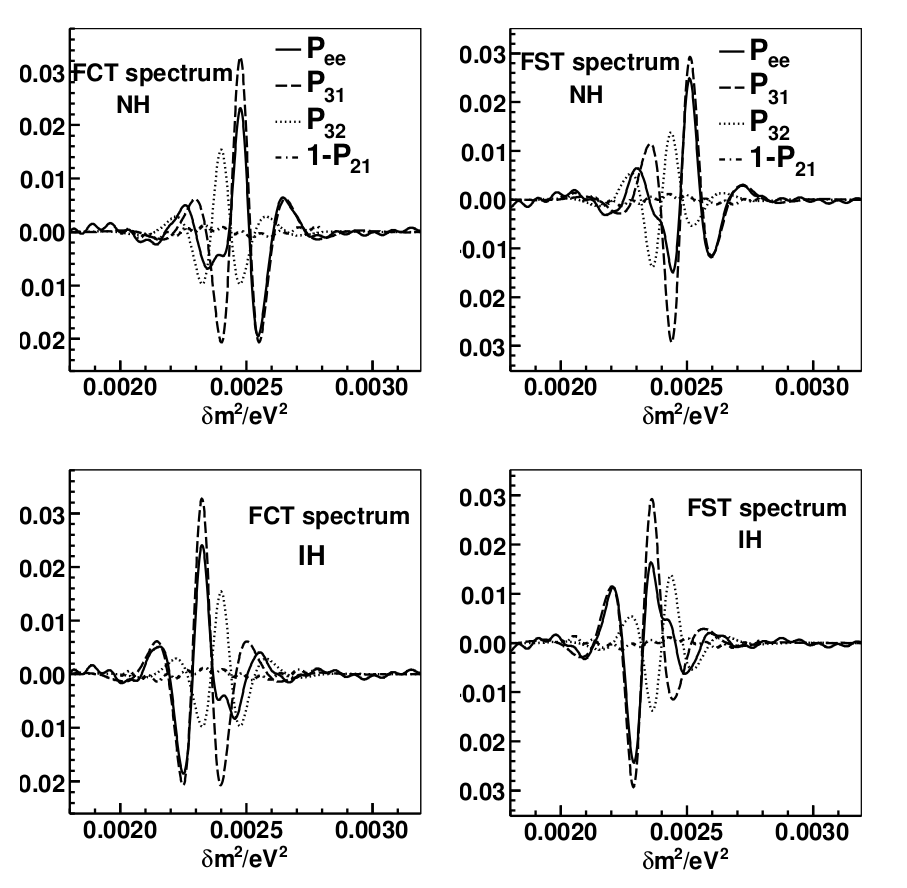
\includegraphics[height=10cm]{images/diff-P31-P32.png}
 \caption{FCT与FST后,三个分量$1-P_{21}$,$P_{31}$,$P_{32}$,的频率谱。横坐标为$\delta m^2$表示质量差平方的差。对比NH和IH在相同$\delta m^2$坐标下的表现,可以将质量顺序区分开。}
 \label{fig:1}
\end{figure}


在NH中,$|\Delta m_{31}^2|=|\Delta m_{32}^2|+|\Delta m_{21}^2|$;在IH中,$|\Delta m_{31}^2|=|\Delta m_{32}^2|-|\Delta m_{21}^2|$,其中$|\Delta m_{31}^2|=(2.13 \pm 0.13) \times 10^{-3}{eV}^2 $。从Figure \ref{fig:1}中可以得到,$P_{31}$,$P_{32}$在$|\Delta m_{32}^2|$和$|\Delta m_{31}^2|$附近有形状比较相似的峰,且在峰的两侧有两个谷,两者的峰之间有一段差值;在FST谱中,其谱线零点的位置对应了FCT谱的峰的位置。将$1-P_{21}$,$P_{31}$,$P_{32}$的FCT和FST谱进行叠加,可以得到NH和IH的FCT和FST谱,将叠加各分量后的FCT和FST谱绘制到一张谱图中如Figure \ref{fig:2}\cite{2009Experimental}:
\begin{figure}[H]
 \centering
 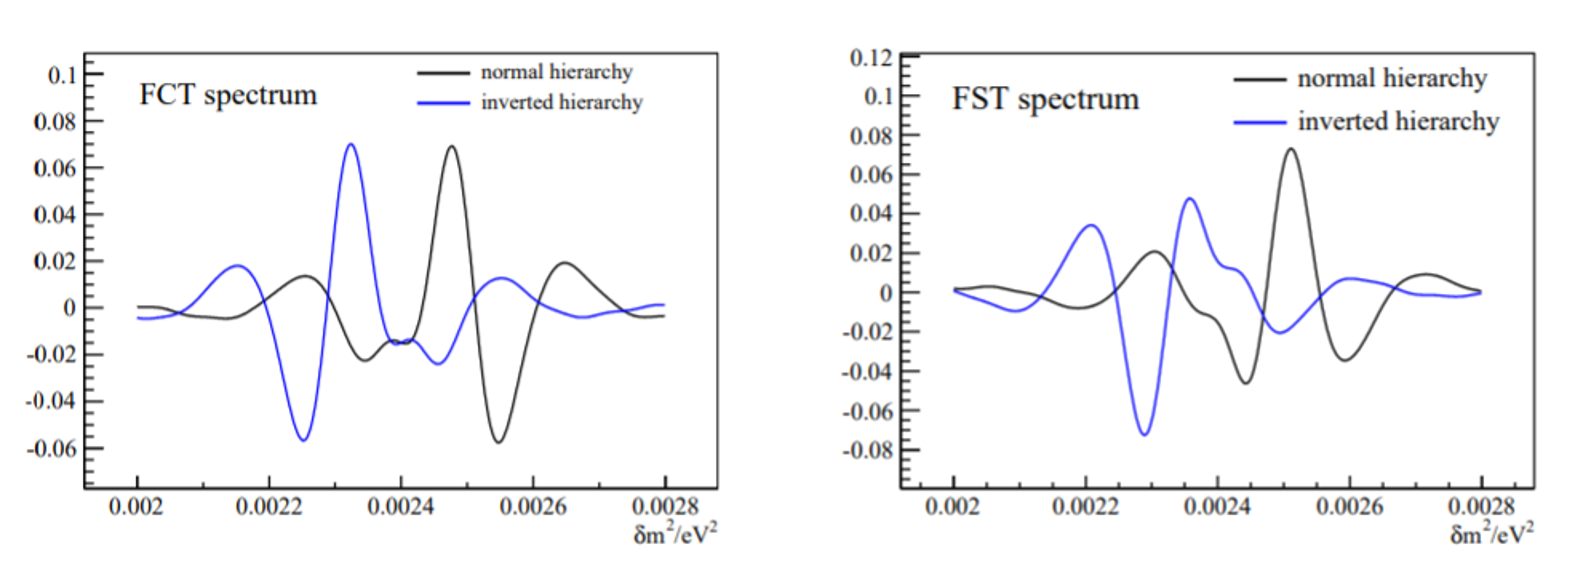
\includegraphics[height=5cm]{images/傅里叶图谱.png}
 \caption{反应堆反中子能谱的傅立叶余弦变换(FCT)(左图)和傅立叶正弦变换(FST)(右图)。黑线和蓝线分别代表NH和IH。}
 \label{fig:2}
\end{figure}

从Figure \ref{fig:2}中可以得到:
\begin{itemize}
	\item{在FCT谱中,NH会在0.0025左右出现一个明显的峰,且在峰的两侧会有两个谷,在峰之后出现的谷比较低。}
    \item{在FCT谱中,IH会在0.0023左右出现一个明显的峰,且在峰的两侧会有两个谷,在峰之前出现的谷比较低。}
    \item{在FCT谱中,NH和IH呈现出关于0.0024轴对称,且对称轴的峰前为IH的,对称轴后的峰为NH的峰。}
    \item{在FCT谱中,NH会在0.0025左右出现一个明显的峰,且在峰的两侧会有两个比较小的谷,在峰之前出现的谷比较低。}
    \item{在FCT谱中,IH会在0.0023左右出现一个明显的谷,且在峰的两侧会有两个比较小的峰,在谷之后出现的峰比较低。}
    \item{在FCT谱中,NH和IH呈现出关于(0.0024,0)中心对称,且对称点前为IH的谷,对称轴后为NH的峰。}
\end{itemize}

为了表征以上的特征,定义两个变量:
\[
RL=\frac{RV-LV}{RV+LV},
PV=\frac{P-V}{P+V}
\]

其中,$RV$表示在FCT谱中右侧谷的幅度,$LV$表示在FCT谱中左侧谷的幅度;$P$表示在FST谱中峰的幅度,$V$表示FST谱中谷的幅度。若质量顺序为NH,则$RL>0$,$PV>0$;若质量顺序为IH,则$RL<0$,$PV<0$。由此,可以在$RL$和$PV$中展开\footnote{目前实验给出的$\sin^2 2\theta_{13}$测量结果可在\cite{Zhan:2008id} TABLE 1中找到;由于测量结果给出的是一定置信水平的置信区间,则该$\sin^2 2\theta_{13}$可在该区间内取不同值进行计算,验证该值是否会对质量顺序的判断带来影响。},得到如Figure \ref{fig:33}:

\begin{figure}[H]
 \centering
 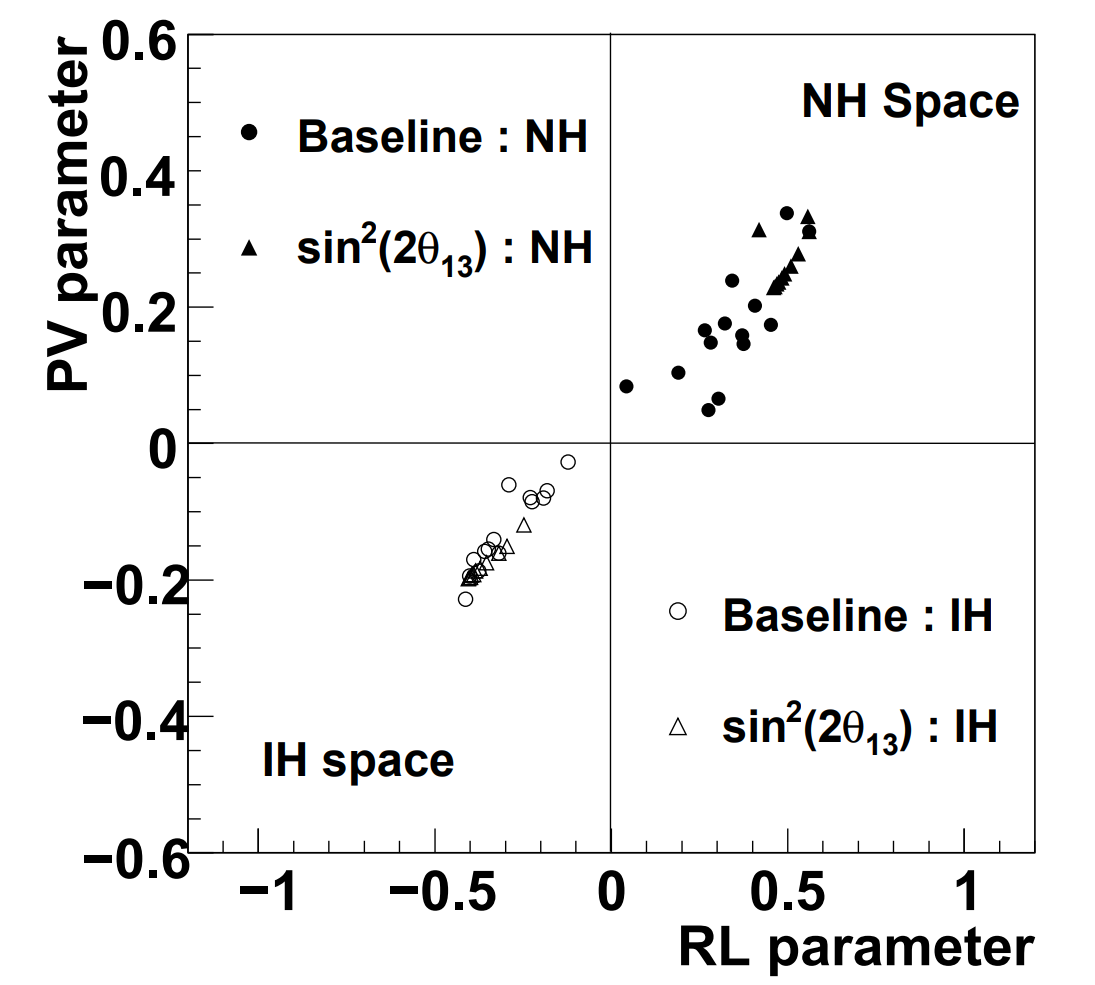
\includegraphics[height=8cm]{images/PVRL.png}
 \caption{取不同的baseline和$\sin^2 2\theta_{13}$,分别计算NH和IH的$RV$和$LV$,并绘制到图像中。}
 \label{fig:33}
\end{figure}


因此,在实验中,可以通过观测探测到的中微子的存活概率的谱,并投射到傅里叶的频率空间,通过对比FST和FCT谱的峰和谷的位置和计算模型中的峰和谷的符合程度,并计算$RL>0$、$PV>0$,判断其位置和符号,对中微子的质量顺序进行判断。


中基线的JUNO中微子实验测量$|\Delta{m_{ee}^2}|$。而:
\begin{equation}
\label{con:eq31}
|\Delta{m_{ee}^2}|-|\Delta {m^{2}_{\mu \mu}}|=\pm \Delta m_{21}^2(\cos2\theta_{12}-\sin2\theta_{12}\sin\theta_{13}\tan\theta_{23}\cos\delta
\end{equation}


式\eqref{con:eq31}中的正负号与质量顺序相关。当与$|\Delta{m_{\mu\mu}^2}|$的测量结合时,可以得到更多关于MH的信息,这使得JUNO实验中,对于MH的测量显得更加的准确\cite{2016Neutrino}。

\subsubsection{JUNO 对中微子的精确测量}\label{sub:1}

除了中微子的质量顺序问题,JUNO实验还将关注中微子振荡参数的精确测量以及测试三中微子标准模型。其具体的工作目标如下\cite{2009Experimental}:

\begin{itemize}
	\item{第一次同时观察由大气和太阳中微子质量平方差驱动的中微子振荡的实验。}
    
    \item{对中微子振荡参数:$\sin^2{\theta_{12}}$,$\Delta m^2_{21}$,$|\Delta m^2_{ee}|$进行高精度的测量,且测量精度优于1\%。}
\end{itemize}


\subsubsection{JUNO其他相关中微子研究}

JUNO实验设备是目前世界上正在建设的最大的液闪探测器,优秀的分辨率和探测精度使得JUNO可以胜任很多的中微子研究。在太阳中微子研究、漫射超新星中微子背景、超新星中微子、大气中微子、地球中微子方面,都将在投入运行采数后发挥重要作用。

\subsection{实验方案}\label{sub:2}

\subsubsection{JUNO的中微子信号}\label{sub:3}

中微子是不带电的粒子,在实验上无法直接观测到,但是中微子会参与一些弱相互作用,产生特定的带电粒子,实验上通过观测中微子与物质作用后产生的次级粒子,可以间接的观测到中微子的信号。

JUNO是通过反$\beta$衰变(inverse beta decay,简称IBD)事件探测中微$$p+\bar{\nu}\Rightarrow e^{+}+n$$
当一个反中微子与质子作用后,会产生一个中子和一个正电子。正电子是空间中不稳定的存在,它会和物质中的电子发生湮灭过程,一个正电子和电子湮灭后会产生两个能量大小为0.511MeV的$\gamma$光子。

在衰变产生中子之后一段时间,中子会被氢原子核俘获,这个过程使得原子核激发,在退激发的过程中会释放一个光子,光子的能量大概是\SI{2.2}{MeV}。


如果探测器探测到这个中微子入射并与液闪作用,那么会在探测得到的波形中看到两个具有时间相关性的不同能量的峰,发生时间早的正电子湮灭过程会先在光谱上的\SI{0.511}{MeV}处或者\SI{1.022}{MeV}处(两个$\gamma$光子发生了重叠)形成观测峰,之后的200多ns后,释放\SI{2.2}{MeV}光子的过程也会完成,在信号的能量谱上形成\SI{2.2}{MeV}处的峰。可以通过做时间符合的方式来进行中微子的信号鉴别,取出中微子的信号。

\subsubsection{实验的探测器设计}\label{sub:4}

江门中微子实验使用的是球体液闪探测器,装载着\SI{20}{kton}液体闪烁体的中心探测器放置在水池中,其建设结构如下Figure \ref{fig:3}:\cite{Ludhova:2020vxz}
\begin{figure}[H]
 \centering
 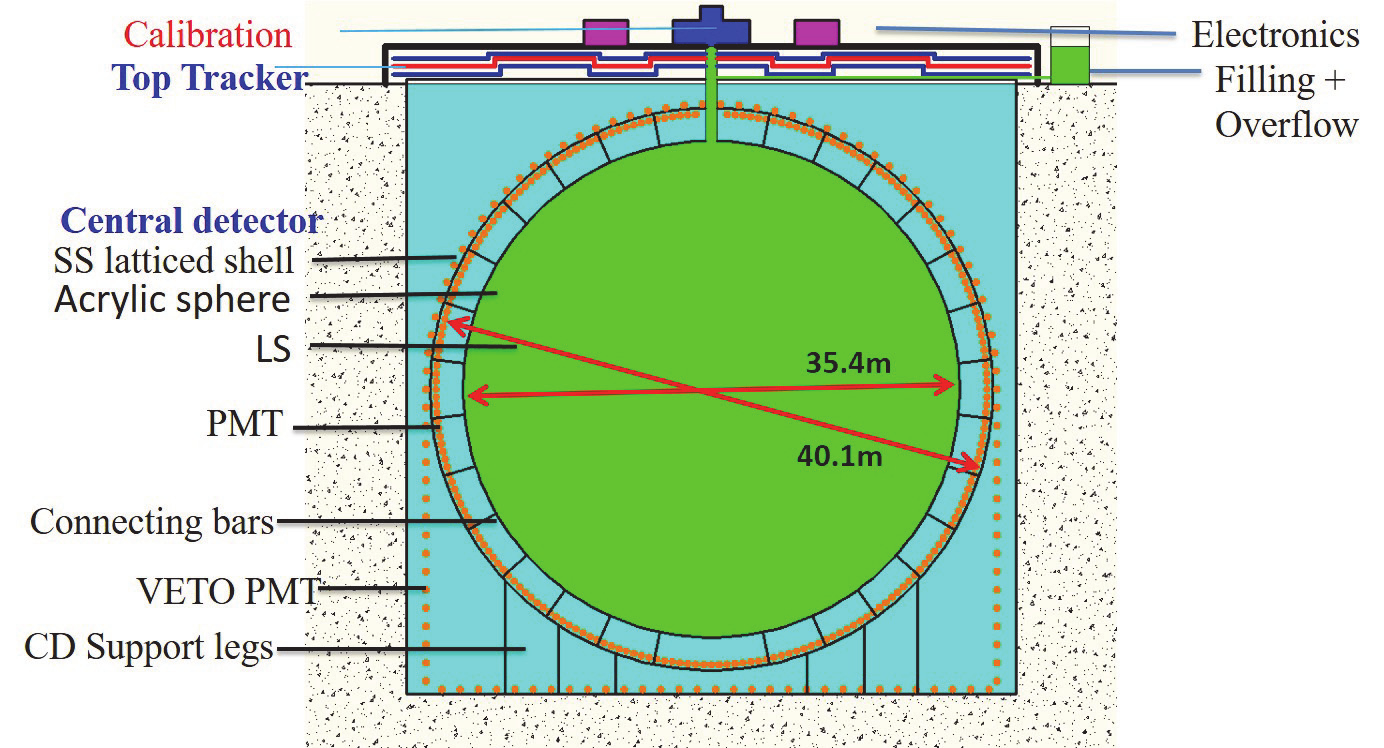
\includegraphics[height=7cm]{images/探测器示意图.png}
 \caption{液闪探测器示意图}
 \label{fig:3}
\end{figure}

中心探测器的表面覆盖了4万多个光电倍增管,其中,18000个光电倍增管的直径为20英寸,分为13000个Micro-channel plates (NNVT)光电倍增管;5000个Dynode光电倍增管( the Hamamatsu R12860 HQE );20寸的光电倍增管具有27\%的探测效率。NNVT光电倍增管具有更小的余波出现概率、玻璃壳带来的本底更低;R12860光电倍增管有更小的渡越时间离散。\cite{Steiger:2019khq}而36000只3英寸的光电倍增管将作为独立的量热器使用。20英寸与3英寸的光电倍增管的镶嵌结构如Figure \ref{fig:22}:
\begin{figure}[H]
 \centering
 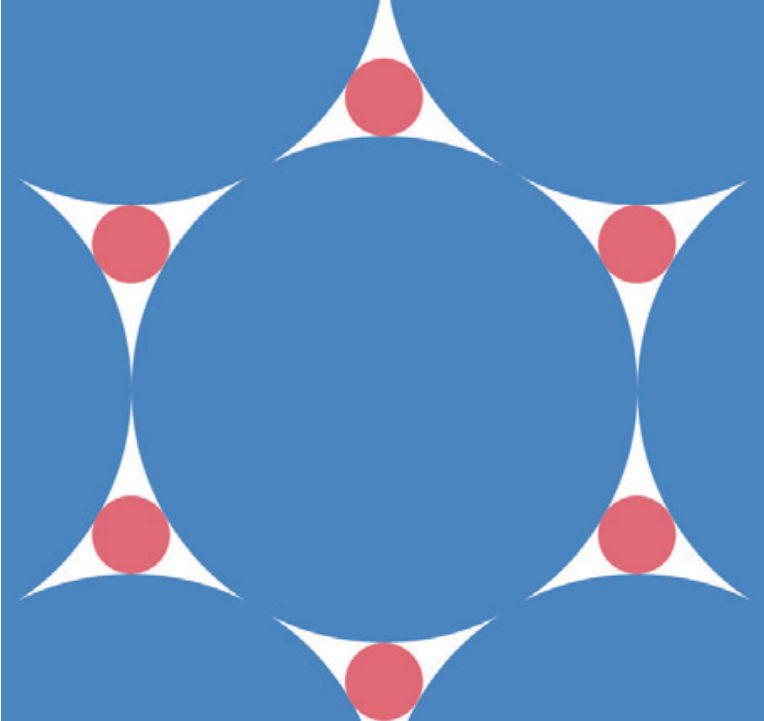
\includegraphics[height=5cm]{images/PMTsyt.png}
 \caption{20英寸的光电倍增管密排,并将3英寸的光电倍增管镶嵌在20英寸管子形成的空隙中。\cite{Zhang:2017ewk}}
 \label{fig:3}
\end{figure}



这些光电倍增管在经过测试后装备使用,在测试中,确定了电荷分辨率、单PE峰谷比、增益为$10^7$所需的工作电压、暗计数率(DCR)、单PE上升和下降时间以及预脉冲和后脉冲率。截至2019年7月已经测试的PMTs的PDE如Figure \ref{fig:4}所示\cite{Steiger:2019khq}。


\begin{figure}[H]
 \centering
 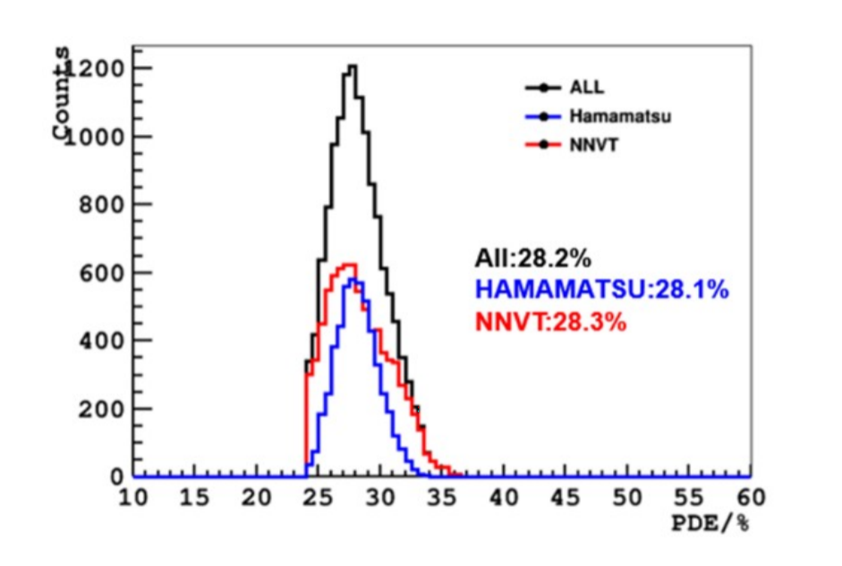
\includegraphics[height=6cm]{images/pmt测试.png}
 \caption{20英寸PMT的PDE测试结果,红色曲线为NNVT管,蓝色为Hamamatsu管,黑色为二者之和。}
 \label{fig:4}
\end{figure}


探测器中装载了20kton的液体闪烁体介质,其中包含的成分为\SI{2.5}{g/L}的PPO和1-\SI{4}{mg/L}的bis-MSB,前者为产生光子的主要成分,后者能将光子的波长进行一定的移动,提高液闪探测器的透光率。

\subsubsection{JUNO的刻度系统}\label{sub:5}
由信号的形成原理可以知道,JUNO实验是通过正电子的快信号和中子的慢信号做符合的方式来确定中微子信号。为了满足实验的高精度要求及正常工作,必须对实验探测器的能量响应和其随空间的变化做精确的标定。对探测器的标定内容通常需要包括:液闪的光学性质、探测器对中子的响应、探测效率以及俘获时间、探测器对于正电子响应、能量标度以及触发等。

JUNO实验有自己的一套刻度系统。主要包括了 Automatic Calibration Unit (ACU),
Cable Loop System (CLS),Guide Tube Control System(GTCS) and Remotely Operated under-liquidscintillator Vehicles (ROV)系统。不同刻度系统的作用如Figure \ref{fig:41}:

\begin{figure}[H]
 \centering
 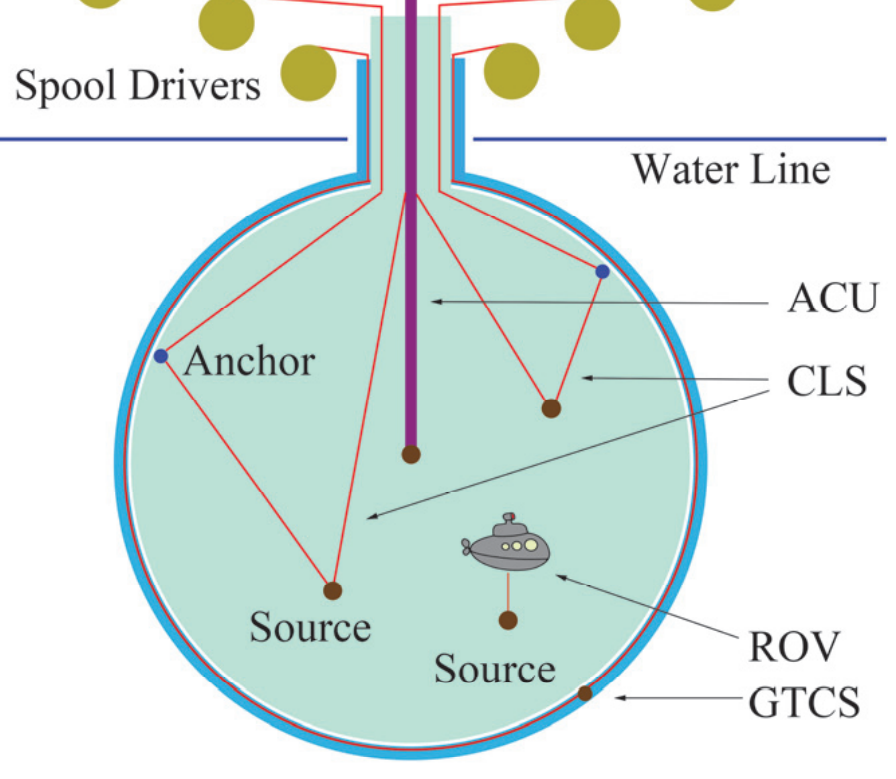
\includegraphics[height=7cm]{images/刻度系统.png}
 \caption{JUNO的刻度系统示意图:ACU是沿着轴线的一维刻度校准系统;CLS和GTCS为平面的二维刻度校准系统,CLS为给定平面的二维刻度校准系统,GTCS为沿着给定经度的亚克力球面的二维刻度校准系统;ROV为人工放置可移动放射源的三维刻度校准系统。}
 \label{fig:41}
\end{figure}

\subsubsection{JUNO TAO(台山反中微子观测台)}\label{sub:6}

台山反中子观测台也是属于JUNO实验的一部分,使用的也是液体闪烁体探测器。

其目标在于精确测量反应堆中微子谱,为JUNO提供独立光谱参考;提供同位素产额和光谱,监控台山核反应堆;同时,它还要用于探测惰性中微子。

台山观测台使用的也是液体闪烁体探测器,其中心探测器是容纳\SI{2.6}{kton}液体闪烁体、直径为\SI{1.7}{m}的球体容器;液闪是掺入一定量的Gd的,工作温度控制在\SI{-50}{℃};表面光电倍增管的覆盖面积超过90\%,光子的探测率超过50\%。\cite{Abusleme:2020bzt}

\begin{figure}[H]
 \centering
 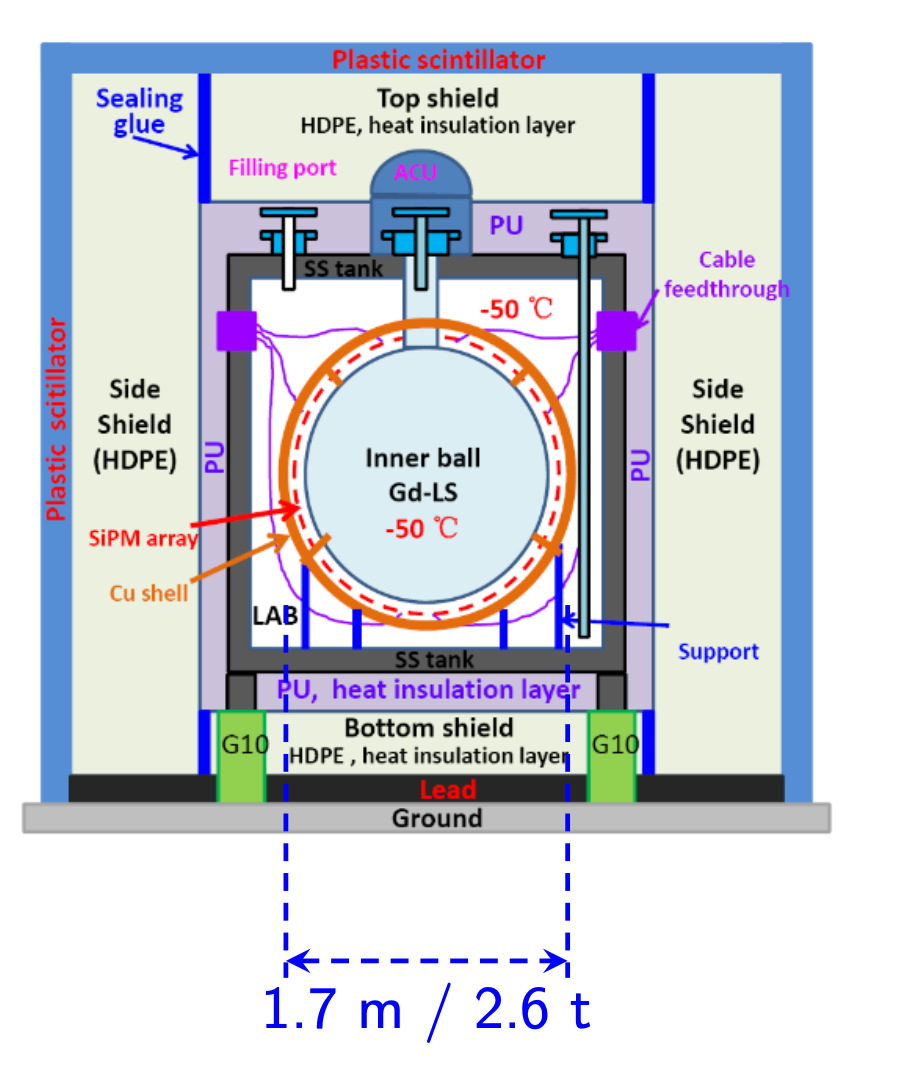
\includegraphics[height=7cm]{images/TAO探测器示意图.png}
 \caption{TAO探测器结构示意图}
 \label{fig:40}
\end{figure}



\subsubsection{JUNO 优势及物理意义}\label{sub:7}

JUNO实验主要依赖周围的核电站的中微子信号进行探测。在距离JUNO50多公里的地方,有阳江核电站和台山核电站,两个核电站功率达到了\SI{26.6}{GW},每天能探测到大概60个来自核反应堆的IBD事件。同时,JUNO对于其他来源的中微子也有足够的探测率:每天能探测到10-1000个太阳中微子,1-2个地球中微子,数个大气中微子。

在1-\SI{8 }{MeV}区间上,JUNO探测器的能量分辨率小于$\frac{3\%}{\sqrt{E}}$且能量探测的不确定度不到1\%,高精度的测量为解决中微子的质量排序问题提供了条件。

目前来说,JUNO实验设备正在建设中,其建设工作预计在2021年完成,投入使用。JUNO实验的开展,将进一步帮助科学家们了解微观粒子的相互作用。

\newpage

\bibliographystyle{unsrt}
\bibliography{ref.bib}

\end{document}


